\documentclass{standalone}
\usepackage{tikz}
\usepackage{ctex,siunitx}
\setCJKmainfont{Noto Serif CJK SC}
\usepackage{tkz-euclide}
\usepackage{amsmath}
\usetikzlibrary{patterns, calc,3d}
\usetikzlibrary {decorations.pathmorphing,decorations.pathreplacing,decorations.shapes}
\tikzset{label style/.append style={font=\small}}
\begin{document}
\small
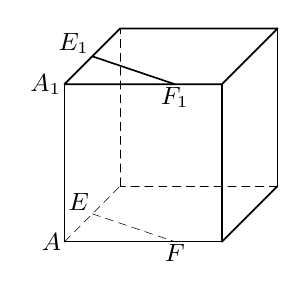
\begin{tikzpicture}[>=latex,scale=1.0,inner sep=1pt]
  \tkzDefPoints{0/0/A,2/0/B,2.707/0.707/C,0.707/0.707/D,0/2/A'}
  \tkzDefPointsBy[translation=from A to A'](B,C,D){B',C',D'}
  \tkzDefMidPoint(A',D')\tkzGetPoint{E'}
  \tkzDefPointOnLine[pos=0.7](A',B')\tkzGetPoint{F'}
  \tkzDefMidPoint(A,D)\tkzGetPoint{E}
  \tkzDefPointOnLine[pos=0.7](A,B)\tkzGetPoint{F}
  \tkzDrawPolygon[semithick](A',B',C',D')
  \tkzDrawSegments[semithick](A,A' B,B' C,C' A,B B,C E',F')
  \tkzDrawSegments[densely dashed](A,D D,D' C,D E,F)
  \tkzLabelPoints[above left](E)
  \tkzLabelPoints[left](A)
  \tkzLabelPoints(F)
  \tkzLabelPoint[left](A'){$A_1$}
  \tkzLabelPoint[above left](E'){$E_1$}
  \tkzLabelPoint(F'){$F_1$}
\end{tikzpicture}
\end{document}